%Grundlagen\\
%- äußere Schalenelektronen für gewöhnlich nach Boltzmann (thermisch) verteilt\\
%- optisches Pumpen sorgt für nicht-thermische Verteilung\\
%
Ein Atom hat diskrete Energieniveaus, auf denen sich die Hüllenelektronen befinden.
Die Verteilung der Elektronen erfolgt bei den äußeren Hüllenelektronen statistisch nach Boltzmann.
Die temperaturabhängigen Besetzungszahlen $N_{1}, N_{2}$ zweier Niveaus mit der statistischen Gewichtung $g_{1}, g_{2}$ und den Energien $W_{1}$, $W_{2}$ ($W_{1}$<$W_{2}$), der Boltzmann-Konstante $k_\text{B}$, der Temperatur $T$ liegen in folgendem Zusammenhang:
\begin{equation*}
  \frac{N_{2}}{N_{1}} = \frac{ g_{2} \exp{  \left( -\frac{W_{2}}{k_{\text{B}} T}  \right) }}{ g_{1} \exp{ \left( -\frac{W_{1}}{k_{\text{B}} T } \right) }}.
\end{equation*}
$k_{\text{B}}$ ist hierbei die Boltzmann-Konstante und $T$ beschreibt die Temperatur.
Das Prinzip des optischen Pumpens besetzt die Niveaus entgegen dieser thermischen Verteilung.\\
In diesem Versuch wird das optische Pumpen mithilfe des Zeeman-Effekts durchgeführt.
Die Aufspaltung der Energieniveaus im Rahmen des Zeeman-Effekts und so auch das optische Pumpen ist abhängig von den quantenmechanischen Eigenschaften der Atome.
%
%Landé-Faktor\\
%- Materialeigenschaft -> Materialbestimmung über diese Messung möglich\\
%- Verhältnisfaktor für das magnetische Moment von Spin, Bahndrehimpuls, etc. zum Bohrschen Magneton\\
%- Bohrsches Magneton: magnetisches Moment für Elektron mit l=1????\\
%- Herleitung: Winkelbeziehungen etc\\
%
\\Der Landé-Faktor $g$ ist eine Materialeigenschaft von Atomen, die zur Stoff- und Isotopenbestimmung benutzt werden kann.
Das Bohr'sche Magneton ist der Betrag des magnetischen Momentes $\vec{\mu}$ eines Elektrons mit Bahndrehimpuls $L=1$.
Der Landé-Faktor ist ein Verhältnisfaktor für die magnetischen Momente des Spins $\vec{S}$, des Bahndrehimpulses $\vec{L}$, des Gesamtdrehimpulses $\vec{J}$, etc. zum Bohr'schen Magneton $\mu_{\text{B}}$:
Das magnetische Moment zu dem Spin $\vec{S}$ sieht wie folgt aus:
\begin{align*}
  \vec{\mu_{\text{S}}} = - g_{\text{S}} \mu_{\text{B}} \vec{S} && \text{mit} && |\vec{\mu_{\text{S}}}|= g_{\text{S}} \mu_{\text{B}} \sqrt{S(S+1)}.\\
\end{align*}
Entsprechend ist das magnetische Moment des Bahndrehimpuls $\vec{L}$
\begin{align*}
  \vec{\mu_{\text{L}}} = - \mu_{\text{B}} \vec{L} && \text{mit} && |\vec{\mu_{\text{L}}}|= \mu_{\text{B}} \sqrt{L(L+1)}.
\end{align*}
\begin{figure}[h!]
  \centering
  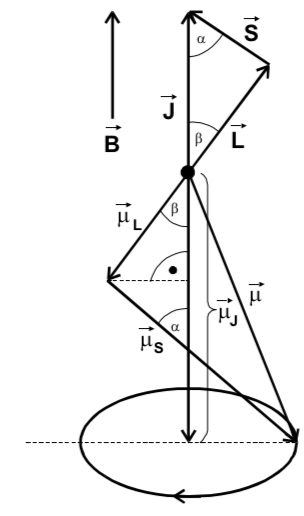
\includegraphics[width=0.3\textwidth]{magmom1.png}
  \caption{Darstellung der verschiedenen magnetischen Momente von Spin, Bahndrehimpuls und Gesamtdrehimpuls \cite{1}}
  \label{fig:magmom}
\end{figure}
Die Kopplung von Spin und Bahndrehimpuls ergibt den Gesamtdrehimpuls $\vec{J}$ der Elektronenhülle und das zugehörige magnetische Moment $\vec{\mu_{\text{J}}}$:
\begin{align*}
  \vec{\mu_{\text{J}}} = \vec{\mu_{\text{S}}} + \vec{\mu_{\text{L}}}= - g_{\text{J}} \mu_{\text{B}} \vec{J} && \text{mit} && |\vec{\mu_{\text{J}}}|=  g_{\text{J}} \mu_{\text{B}} \sqrt{J(J+1)}.
\end{align*}
Nur das magnetische Moment $|\vec{\mu_{\text{J}}}|$ in Richtung von $\vec{J}$ hat einen Effekt auf die Energiebilanz, da das magnetische Moment eine Präzessionsbewegung um $\vec{J}$ vollführt (Abb. \ref{fig:magmom}) und sich die senkrechten Komponenten herausmitteln.
Die Winkelbeziehung in $|\vec{\mu_{\text{J}}}|$ lässt sich aus Abbildung \ref{fig:magmom} erkennen.
Damit ergibt sich:
\begin{align*}
                   |\vec{\mu_{\text{J}}}|                    =  |\mu_{\text{S}}| \cos{(\alpha)}                          + |\mu_{\text{L}}| \cos{(\beta)} \\
 \Leftrightarrow   g_{\text{J}} \mu_{\text{B}} \sqrt{J(J+1)} = g_{\text{S}} \mu_{\text{B}} \sqrt{S(S+1)} \cos{(\alpha)}  + \mu_{\text{B}} \sqrt{L(L+1)} \cos{(\beta)}
\end{align*}
Für die Winkel lässt sich aufstellen:
\begin{align*}
  \cos{(\alpha)} = \frac{ |\vec{S}|^2 - |\vec{L}|^2 + |\vec{J}|^2}{2 |\vec{L}||\vec{J}|^2} \\% &=& \frac{ \left(g_{\text{S}} \mu_{\text{B}} \sqrt{S(S+1)}\right)^2  -  \left( \mu_{\text{B}} \sqrt{L(L+1)} \right)^2  +  \left( g_{\text{J}} \mu_{\text{B}} \sqrt{J(J+1)} \right)^2 }{  2              \mu_{\text{B}} \sqrt{L(L+1)} g_{\text{J}} \mu_{\text{B}} \sqrt{J(J+1)}    } \\
  \cos{(\beta)}  = \frac{-|\vec{S}|^2 + |\vec{L}|^2 + |\vec{J}|^2}{2 |\vec{S}||\vec{J}|^2}.\\% &=& \frac{-\left(g_{\text{S}} \mu_{\text{B}} \sqrt{S(S+1)}\right)^2  +  \left( \mu_{\text{B}} \sqrt{L(L+1)} \right)^2  +  \left( g_{\text{J}} \mu_{\text{B}} \sqrt{J(J+1)} \right)^2 }{  2 g_{\text{S}} \mu_{\text{B}} \sqrt{S(S+1)} g_{\text{J}} \mu_{\text{B}} \sqrt{J(J+1)}    }.\\
\end{align*}
Es ergibt sich:
\begin{equation}
  g_{\text{J}}= \frac{\left(g_{\text{S}} +1 \right)J\left(J+1\right) + \left(g_{\text{S}}-1\right) \left[ S\left(S+1\right)-L\left(L-1\right) \right]   }{2J\left(J+1\right)}.
\label{eqn:landej}
\end{equation}
%
%Zeeman-Effekt\\
%- Aufspaltung der Hyperfeinstruktur durch ein äußeres Magnetfeld\\
%- Aufspaltung proportional zum Landé-Faktor\\
%
\\Der Zeemaneffekt beschreibt die Aufspaltung der vorhandenen Energieniveaus durch ein äußeres Magnetfeld.
Die magnetischen Momente wechselwirken mit dem äußeren Magnetfeld $\vec{B}$ und es haben nur die Beiträge entlang der $\vec{B}$-Achse einen Effekt.
Durch die Richtungsquantelung ist die Wechselwirkungsenergie $E_{\text{mag}}$ ein ganzzahliges Vielfaches $M_{\text{J}}$ (Orientierungsquantenzahl) von $g_{\text{J}} \mu_{\text{B}} B$:
\begin{equation}
  E_{\text{Zeeman}} = -\vec{\mu_{\text{J}}} \vec{B} \Rightarrow E_{\text{Zeeman}} = g_{\text{J}} \mu_{\text{B}} M_{\text{J}} B.
  \label{eqn:zeeman}
\end{equation}
Die Orientierungsquantenzahl oder magnetische Quantenzahl $M_{\text{J}}$ kommt aus der Projektion des Bahndrehimpulses auf die z-Achse:
\begin{equation*}
  L_\text{z}= M_{\text{J}} \hbar.
\end{equation*}
Es lässt sich beweisen, dass bei dem Zeemaneffekt nur bestimmte Neigungen des magnetischen Moments $\mu$ zum äußeren Magnetfeld $\vec{B}$ vorhanden sind und damit nur bestimmte Werte von $M_{\text{J}}$ (ganzzahlige Werte) auftreten.
%
%Kernspin\\
%- Eigendrehimpuls des Atomkerns\\
%- neuer Landé-Faktor\\
%\begin{equation}
%  g_{\text{F}}= g_{\text{J}} \frac{ F\left(F+1\right) + J\left(J+1\right) - I\left(I-1\right)  }{2 \sqrt{F\left(F+1\right)}}
%\label{eqn:landef}
%\end{equation}
%
\\Der Kernspin $\vec{I}$ entspricht dem Eigendrehimpuls des Atomkerns und führt zur Aufspaltung der Energieniveaus im Rahmen der Hyperfeinstruktur.
Die Hyperfeinstruktur wird durch den Zeemaneffekt weiter aufgespalten (Abb. \ref{fig:kernspin}).
\begin{figure}[h!]
  \centering
  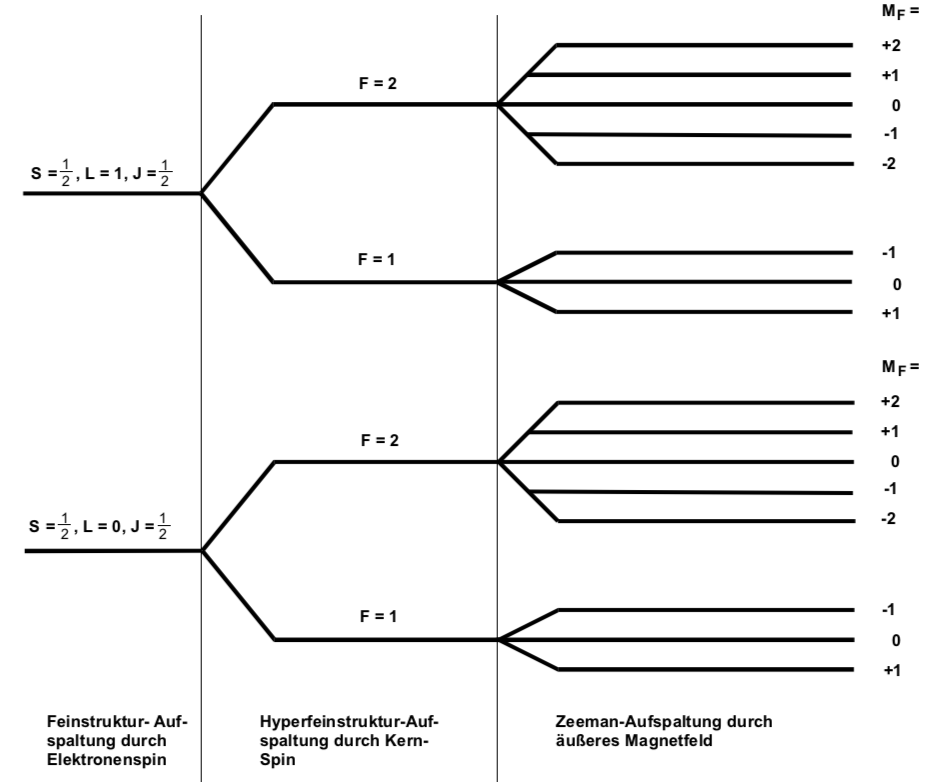
\includegraphics[width=\textwidth]{kernspin1.png}
  \caption{Darstellung der Aufspaltung der Energieniveaus durch die Hyperfeinstruktur und den Zeemaneffekt \cite{1}}
  \label{fig:kernspin}
\end{figure}
Der Gesamtdrehimpuls $\vec{J}$ der Elektronenhülle und der Kernspin $\vec{I}$ koppeln zu dem Gesamtdrehimpuls $\vec{F}$ des Atoms:
\begin{align*}
  \vec{F}=\vec{J}+\vec{I} && mit && |\vec{\mu_{\text{F}}}|= g_{\text{F}} \mu_{\text{B}} \sqrt{F(F+1)}.\\
\end{align*}
Der Kernspin beeinflusst auch den Landé-Faktor $g_{\text{F}}$, der sich nun wie folgt berechnet:
\begin{equation}
  g_{\text{F}}= \frac{F(F+1) + J(J+1) - I(I+1)}{2 F(F+1)}
  \label{eqn:landef}
\end{equation}
%
%Idee des optischen Pumpens\\
%- Übergänge der Elektronen auf den Energieniveaus durch Anregung\\
%- um bestimmte Übergänge zu produzieren, bestimmtes Spektrallicht einstrahlen ($D_{1}$-Licht)\\
%  --- Anregung/Quantensprünge $E_{2}-E_{1}=h \nu$\\
%- um GANZ bestimmte Übergänge zu produzieren, bestimmtes polarisiertes Licht einstrahlen ($\sigma^{+}$-Licht)\\
%  ——- Auswahlregeln\\
%- angeregte Zustände fallen in alle Grundzustände zurück\\
%- $\sigma^{+}$ pumpt (über die genannten Umwege) die Elektronen aus dem niedrigerem Grundzustand in den höheren Grundzustand\\
%
\\Das optische Pumpen basiert auf der Idee, die Elektronen aus ihrer thermischen Verteilung auf den Hüllen zu bringen.
Die verwendeten Stoffe entstammen der Alkali-Gruppe, also haben die Atome immer nur ein Elektron auf der äußersten Schale.
Der Einfachheit halber wird zunächst mit der Annahme gearbeitet, dass das Atom einen Kernspin mit $I=0$ besitzt.
Als Grundzustand ergibt sich somit $^{2}S_{\frac{1}{2}}$.
Die angeregten Zustände sind $^{2}P_{\frac{1}{2}}$ und $^{2}P_{\frac{3}{2}}$.
Die Energieniveaus sind in Abbildung \ref{fig:doublett} dargestellt.
Die beiden Übergänge in Abbildung \ref{fig:doublett} werden $D_{1}$-$D_{2}$-Doublett genannt.
Wird ein äußeres Magnetfeld angelegt, entsteht eine Zeeman-Aufspaltung.
Die Zeeman-Aufspaltung des $D_{1}$-Übergangs ist in Abbildung \ref{fig:sigmaplus} abgebildet.
Bei der Zeeman-Aufspaltung unterscheiden sich die Übergänge durch die Polarisation des Lichts (Tab. \ref{tab:polarisation}).
\begin{table}[h!]
  \centering
  \caption{Übergänge der Zeeman-Aufpaltung}
  \label{tab:polarisation}
  \begin{tabular}{l l l l l r l l r l c l l r l l l l l l l l l l l l}
    \toprule
$\sigma^{+}$ && rechtszirkular && $\Delta M_{\text{J}}=$ & $+1:$  &&  $^{2}P_{\frac{1}{2}},$ $\Delta M_{\text{J}}=$ & $-\frac{1}{2}$ &&$\Rightarrow$&& $^{2}S_{\frac{1}{2}},$ $\Delta M_{\text{J}}=$ & $+\frac{1}{2}$ \\
$\sigma^{-}$ && linkszirkular  && $\Delta M_{\text{J}}=$ & $-1:$  &&  $^{2}P_{\frac{1}{2}},$ $\Delta M_{\text{J}}=$ & $+\frac{1}{2}$  &&$\Rightarrow$&& $^{2}S_{\frac{1}{2}},$ $\Delta M_{\text{J}}=$ & $-\frac{1}{2}$ \\
$\pi       $ && linear         && $\Delta M_{\text{J}}=$ & $ 0:$  &&  $^{2}P_{\frac{1}{2}},$ $\Delta M_{\text{J}}=$ & $+\frac{1}{2}$  &&$\Rightarrow$&& $^{2}S_{\frac{1}{2}},$ $\Delta M_{\text{J}}=$ & $+\frac{1}{2}$ \\
$\pi$        && linear         && $\Delta M_{\text{J}}=$ & $ 0:$  &&  $^{2}P_{\frac{1}{2}},$ $\Delta M_{\text{J}}=$ & $-\frac{1}{2}$ &&$\Rightarrow$&& $^{2}S_{\frac{1}{2}},$ $\Delta M_{\text{J}}=$ & $-\frac{1}{2}$ \\
    \bottomrule
  \end{tabular}
\end{table}
%Wird nun der Stoff spezifisch mit $D_{1}$-Licht angeregt, fällt er nur über den $D_{1}$-Übergang aus dem angeregten $^{2}P_{\frac{1}{2}}$-Zustand zurück in seinen Grundzustand $^{2}S_{\frac{1}{2}}$.
Wird der Stoff mit $\sigma^{+}$-polarisiertem $D_{1}$-Licht angeregt, werden die Elektronen vom $^{2}S_{\frac{1}{2}}, \Delta M_{\text{J}}= -\frac{1}{2}$-Zustand in den $^{2}P_{\frac{1}{2}}, \Delta M_{\text{J}}= +\frac{1}{2}$-Zustand gebracht.
Von dort fallen sie aber in beide Grundzustände $^{2}S_{\frac{1}{2}}, \Delta M_{\text{J}}= \pm \frac{1}{2}$ zurück.
Mit diesem Prinzip gelingt es, den $^{2}S_{\frac{1}{2}}, \Delta M_{\text{J}}= -\frac{1}{2}$-Zustand (energieärmer) leer zu pumpen und den $^{2}S_{\frac{1}{2}}, \Delta M_{\text{J}}= +\frac{1}{2}$-Zustand (energiereicher) voll zu pumpen.
Damit ist das Atom nicht mehr in seiner thermischen Verteilung.
\begin{figure}[h!]
 \centering
 \begin{subfigure}{0.48\textwidth}
  \centering
  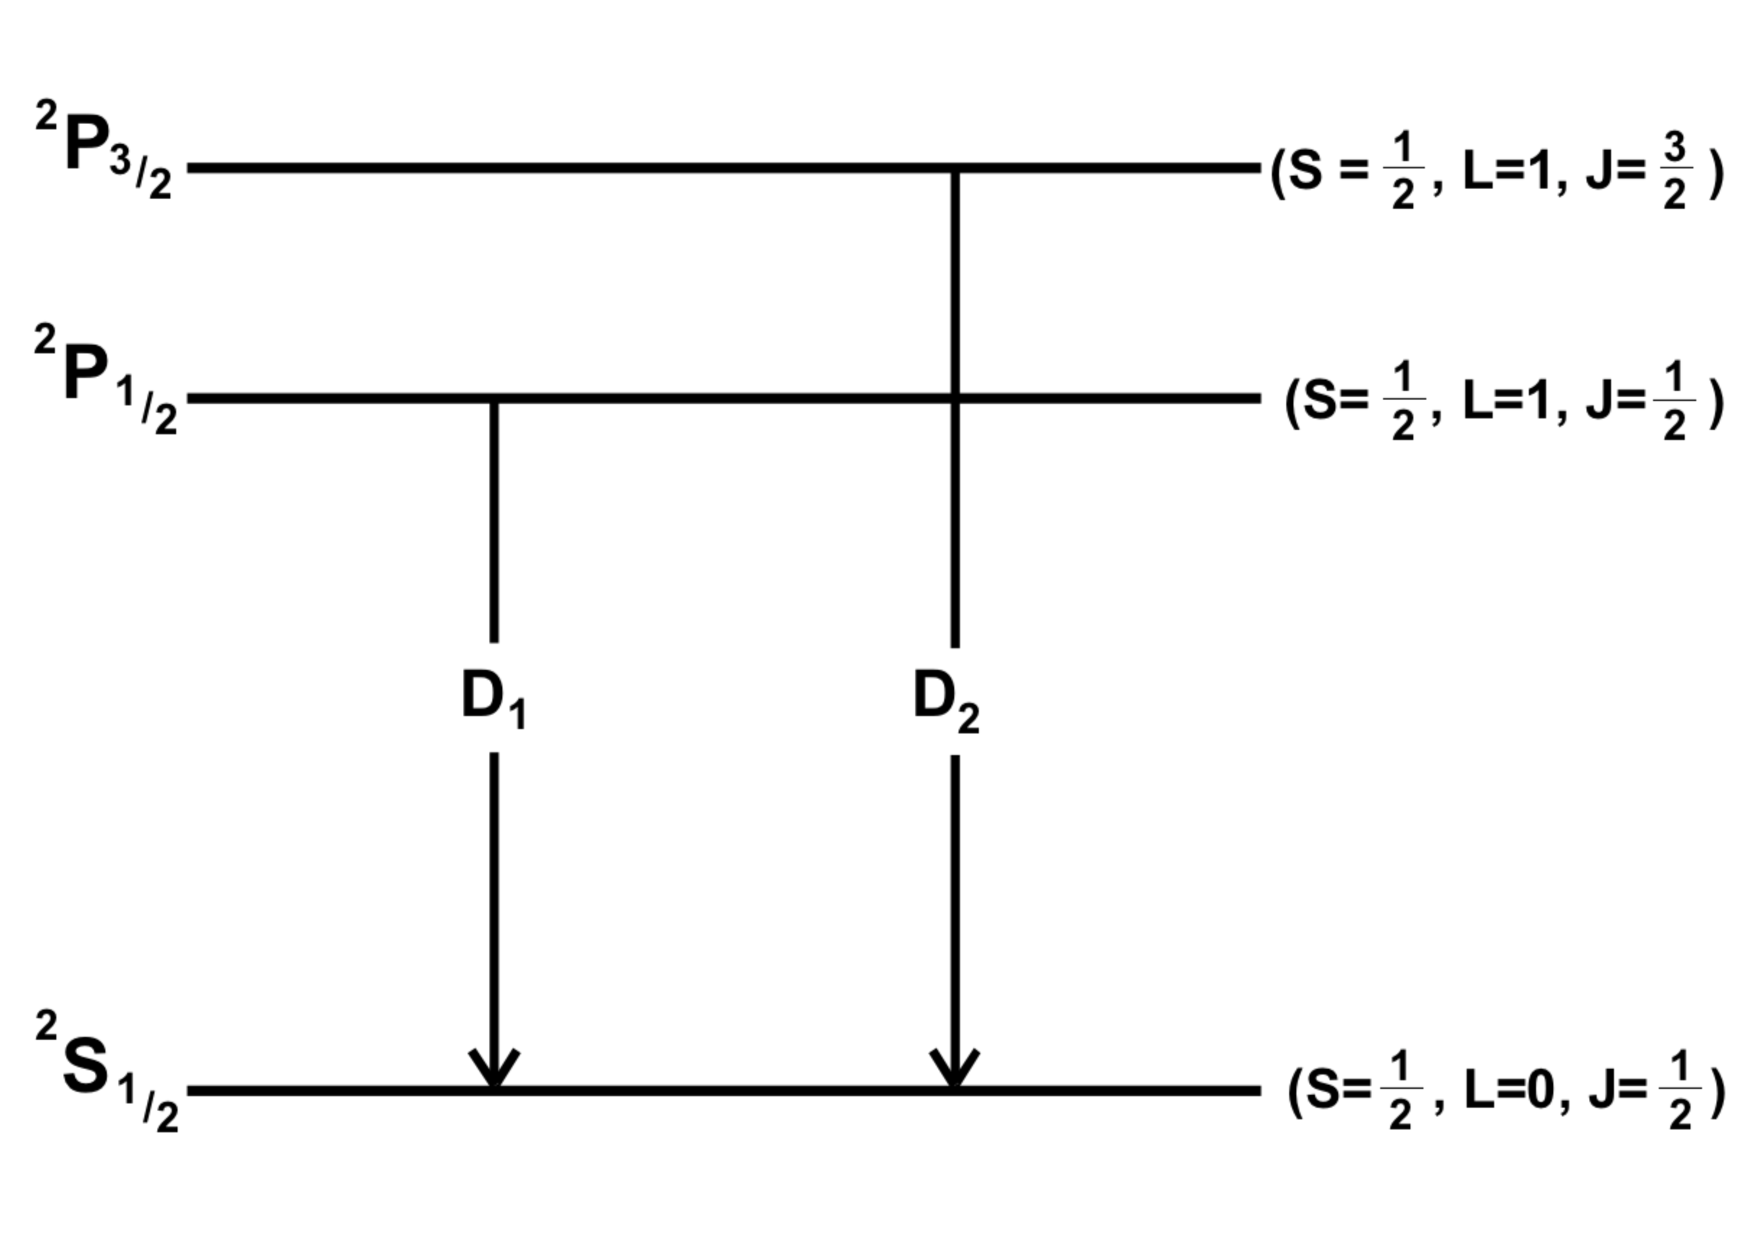
\includegraphics[width=\textwidth]{doublett.pdf}
  \caption{$D_{1}$-$D_{2}$-Doublett eines Alkali-Atoms mit $I=0$}
  \label{fig:doublett}
 \end{subfigure}
 \begin{subfigure}{0.48\textwidth}
  \centering
  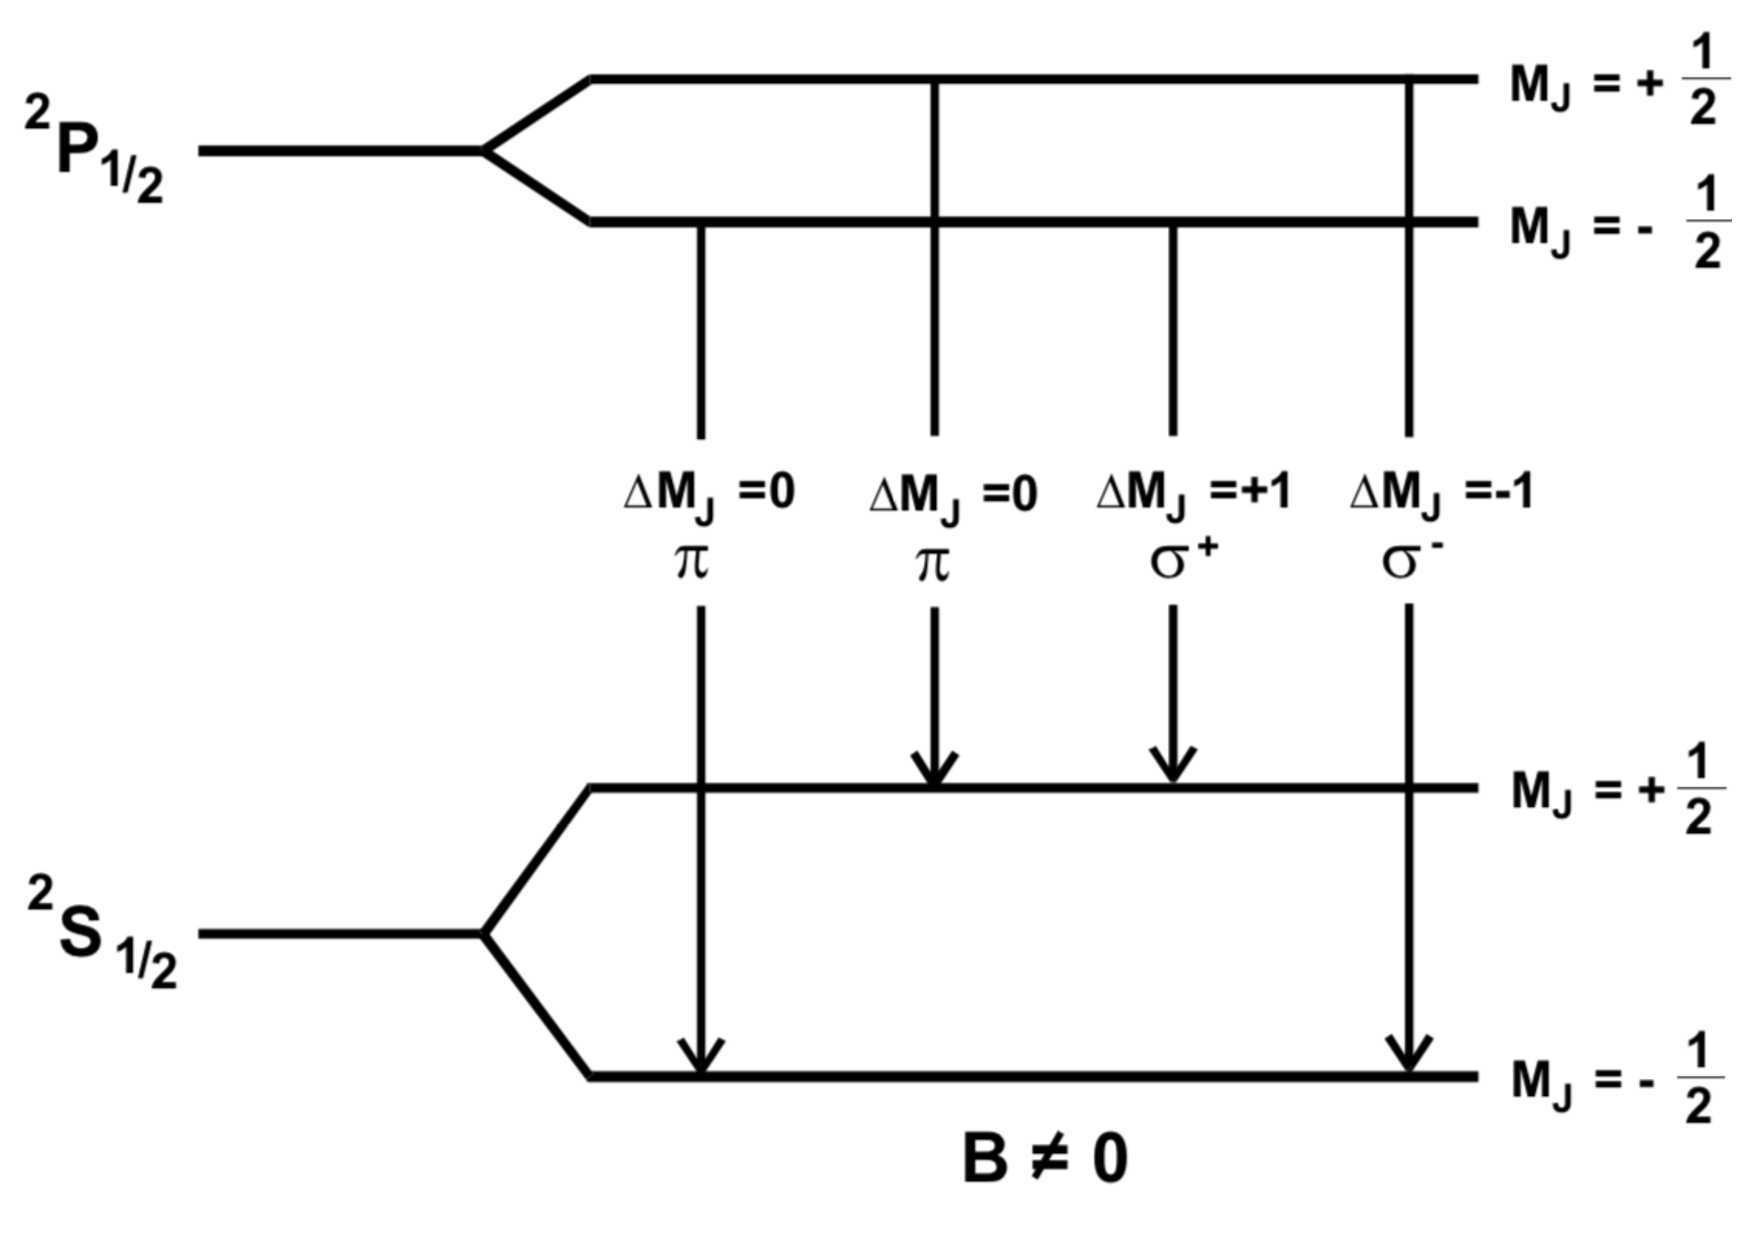
\includegraphics[width=\textwidth]{sigmaplus.pdf}
  \caption{Übergänge der Zeeman-Aufspaltung eines Alkali-Atoms mit $I=0$}
  \label{fig:sigmaplus}
 \end{subfigure}
 \caption{Übergänge eines Alkali-Atoms}
 \label{fig:übergänge}
\end{figure}
%
%Optisches Pumpen + Aufbau\\
%- zunächst sind alle Anregungen möglich, da die Elektronen noch auf allen Niveaus vorhanden sind\\
%- das Licht wird also vollständig absorbiert\\
%- mit der Zeit werden die Elektronen in einem Energieniveau gesammelt\\
%- es sind keine Absorptionen möglich\\
%- das Gas wird zunehmend transparent\\
%
\\Um das optische Pumpen zu messen, lässt sich die Transparenz des verdampften Stoffs beobachten.
Das $\sigma^{+}$-polarisierte $D_{1}$-Licht wird eingestrahlt und trifft auf das Gas.
Initial bei Einschalten des Magnetfelds ist noch Absorption im Gas möglich, da alle Grundzustände gleichmäßig besetzt sind.
Zu Beginn der Messung wird das Licht der Spektrallampe absorbiert, das Gas ist also wenig transparent.
Mit fortlaufender Zeit werden durch das optische Pumpen die Elektronen aus dem energieärmeren Grundzustand in den energiereicheren Grundzustand gepumpt.
Von dort aus können keine weiteren Anregungen ausgehen, und es wird immer weniger Licht der Spektrallampe absorbiert, das Gas wird also zunehmend transparent.
%
%Emission\\
%- spontane Emission: Elektron fällt von alleine zurück (statistisch)\\
%  --- Wahrscheinlich bei hohen Frequenzen des RF-Felds\\
%- induzierte Emission: Elektron fällt zurück entlang der Energie der eingestrahlten Photonen (RF-Quanten)\\
%  --- Wahrscheinlich bei niedrigen Frequenzen des RF-Felds\\
%- induzierte Emission bei 'Resonanzstelle' (passendes RF-Feld mit der richtigen Energie für induzierte Emission)\\
%
\\Für die Messung der Zeeman-Aufspaltung werden zwei weitere Phänomene vorgestellt.
Die spontane Emission bedeutet, dass das Elektron ohne weitere äußere Einwirkung nach gewisser Zeit zurück in den Grundzustand fällt.
Die induzierte Emission entsteht, wenn die Anregungsenergie als Quanten eingestrahlt wird und das Elektron unter Emission der Anregungsenergie bzw. der Quanten in den Grundzustand zurückfällt.
Die induzierte und die spontane Emission können parallel ablaufen.
Parallel wird die Anregungsenergie auch rückabsorbiert.
%Durch ein hochfrequentes veränderliches Magnetfeld (RF-Feld) wird bei diesem Versuch die Anregungsenergie bzw die sogenannten RF-Quanten eingebracht.
Das Verhältnis der beiden Emissionsarten wird über die Anregungsenergie $h \nu$ bestimmt.
Die Anzahlen $n$ der verschiedenen Emissionen pro Zeiteinheit lauten:
\begin{align*}
n_{\text{spon}} &= N_{2} A_{21}        \\
n_{\text{ind}}  &= N_{2} B_{21} u(\nu) \\
n_{\text{abs}}  &= N_{1} B_{12} u(\nu).\\
\end{align*}
Dabei ist $N$ die Atomzahl, $A_{21}$ die Übergangswahrscheinlichkeit der spontanen Emission und $B$ der Einstein-Koeffizient (Proportionalitätsfaktor).
$u(\nu)$ ist die Dichte der eingestrahlten Quanten.
Die drei Gleichungen lassen sich mit der Bedingung $B_{21}=B_{12}$ durch eine Erhaltung der Übergangszahlen verbinden und durch weitere Überlegungen und das Einbringen der Planckschen Gleichung für schwarze Strahler schreiben als:
\begin{equation*}
  n_{\text{spon}} + n_{\text{ind}} = n_{\text{abs}} \Rightarrow A_{21}= \frac{8 \pi h}{c^{3}}B_{12} \nu^{3}.
\end{equation*}
Damit ist die spontane Emission proportional zu $\nu^3$.
Bei höheren Frequenzen des RF-Felds kommt hauptsächlich die spontane Emission vor, bei den niedrigeren Frequenzen kommt die spontane Emission immer weniger vor.
Erreicht das RF-Feld eine passende Frequenz, setzt also die induzierte Emission ein.
Hier bedeutet dies, dass die Elektronen über die induzierte Emission wieder aus der aufgebauten, nicht-thermischen Verteilung gelangen, wenn das RF-Feld die passende Frequenz hat (Abb. \ref{fig:transparenz}).
Das höhere Niveau entleert sich nun, da die induzierte Emission bei der passenden Frequenz möglich ist.
Damit verringert sich im Bereich der passenden Frequenz die Transparenz des Gases, da die Absorptionen wieder möglich sind.
\begin{figure}[h!]
  \centering
  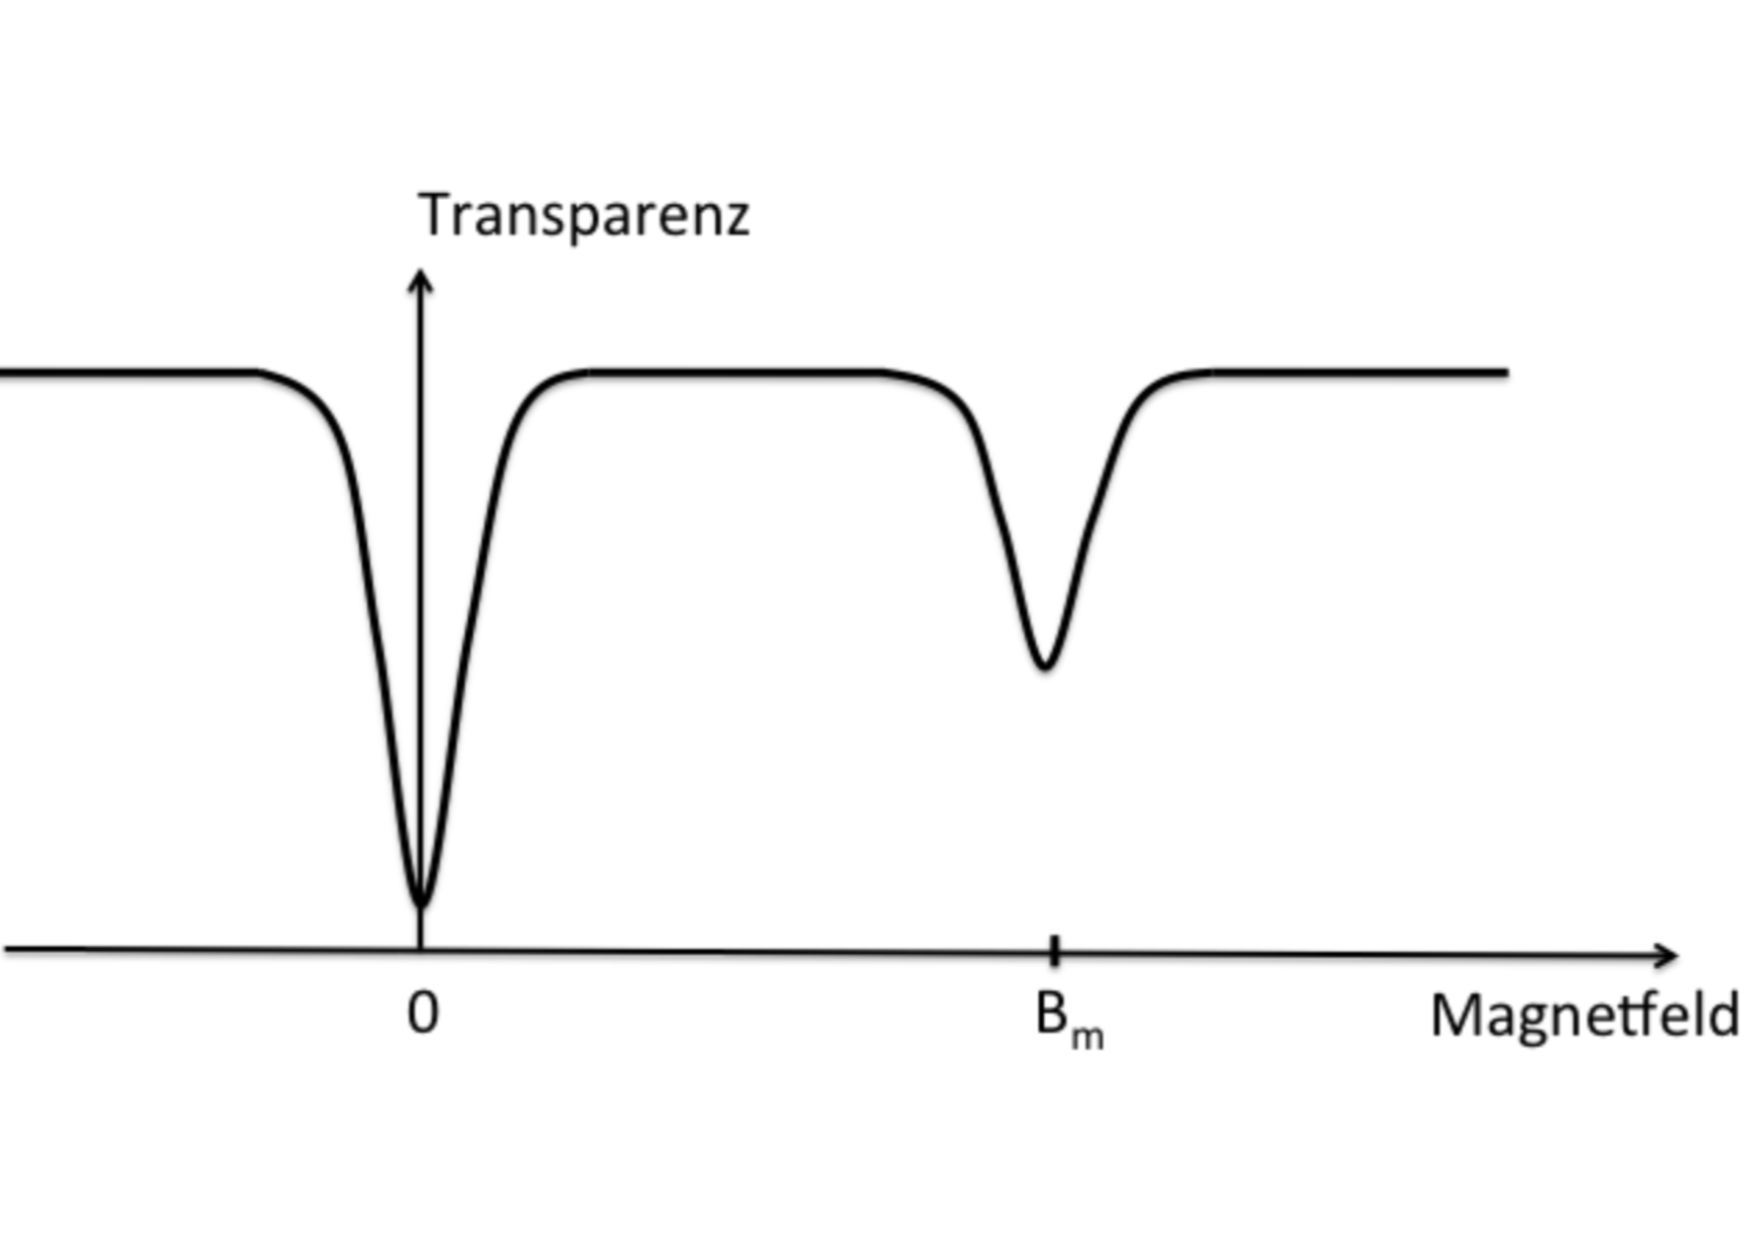
\includegraphics[width=\textwidth]{transparenz.pdf}
  \caption{Transparenz des Gases mit angelegtem RF-Feld und Resonanzstelle \cite{1}}
  \label{fig:transparenz}
\end{figure}
Dies ist mit Gleichung \eqref{eqn:zeeman} der Fall bei:
\begin{equation}
  h \nu = g_{\text{J}} \mu_{\text{B}} \Delta M_{\text{J}} B_{\text{m}} \Leftrightarrow B_{\text{m}} = \frac{4 \pi m_{0}}{e_{0} g_{\text{J}}} \nu.
\label{eqn:resonanz}
\end{equation}
$B_{\text{m}}$ wird auch Resonanzstelle genannt.
%
%Optisches Pumpen + Kernspin\\
%- Energie der Spektrallinie überdeckt alle Hyperfeinstrukturen und Zeemaneffekt\\
%- $\sigma^{+}$-Licht lässt nur $\Delta M_{\text{F}}= +1$ zu, also sammeln sich die Elektronen bei $^{2}S_{1/2}, F=2, M_{\text{F}}=+2$ \\
%
\\Nun wird wieder der Kernspin $I≠0$ in die Theorie gebracht.
Die Energie des $D_{1}$-Lichts überdeckt alle möglichen Übergänge der Hyperfeinstruktur und des Zeemaneffekts (Abb. \ref{fig:übergänge}).
\begin{figure}[h!]
  \centering
  \includegraphics[width=\textwidth]{übers.pdf}
  \caption{Übergänge des $D_{1}$-Lichts mit Betrachtung eines Kernspin $I=\frac{3}{2}≠0$ \cite{1}, bearbeitet}
  \label{fig:übergänge}
\end{figure}
In blau gekennzeichnet sind die Übergänge, die durch die Auswahlregel $\Delta M_{\text{F}}=+1$ möglich sind.
Aus dem Grundzustandsniveau mit $F=2$ und $M_{\text{F}}=+2$ ist kein Übergang in das angeregte Niveau möglich.
Durch spontane Emission (grün gekennzeichnet) können aber Elektronen von den Niveaus $M_{\text{J}}=+1$ und $M_{\text{J}}=0$ in das Niveau $M_{\text{F}}=+2$ übergehen.
So lässt sich dennoch mittels des optischen Pumpens eine nicht-thermische Verteilung erzeugen.
Das Niveau, welches durch das optische Pumpen besetzt wird, ist in diesem Versuch
\begin{align*}
  s= \frac{1}{2}, \quad L = 0, \quad J= \frac{1}{2}, \quad F = 2, \quad \mathbf{M_{F}=2}.
\end{align*}
\FloatBarrier
%
%Quadratischer Zeemaneffekt/Breit-Rabi-Formel\\
%- große B-Felder\\
%- Wechselwirkung Spin-Bahn-Kopplung\\
%- Wechselwirkung magnetische Momente\\
%
Bei starken Magnetfeldern entstehen weitere Effekte, die sich aus der Wechselwirkung des Spins und dem Bahndrehimpuls und der Wechselwirkung der magnetischen Momente ergeben.
Die Zeemanaufspaltung berechnet sich dann über:
\begin{equation}
U_{\text{HF}}= g_{\text{F}} \mu_{\text{B}} B + g_{\text{F}}^2 \mu_{\text{B}}^2 B^2 \frac{(1- 2M_{\text{F}})}{\Delta E_{\text{HF}}}
\label{eqn:quadzeeman}
\end{equation}
und wird quadratischer Zeemaneffekt genannt.
Dabei ist $\Delta E_{\text{HF}}$ die Energiedifferenz zwischen den Energieniveaus mit den Quantenzahlen $F$ und $F+1$.
%Als $M_{\text{F}}$ wird der niedrigere Wert $M_{\text{F}}$ des Übergangs verwendet.
$M_{\text{F}}$ bestimmt sich aus dem jeweiligen Übergang und beschreibt das Niveau, welches hier besetzt wird.
Bei diesem Versuch ist dies, wie bereits beschrieben (Abb. \ref{fig:übergänge}), $M_{F} = 2$.
\FloatBarrier
